% Provenance (never printed): see sources/outline_sources.md (Year 2: oceanic islands; growth,
% flank collapse and erosion of volcanic islands; reefs and atolls; subsidence). Hawaiian
% stages, slides, subsidence and drowned reefs after Clague and Sherrod (2014, USGS PP 1801
% ch. 3) and Denlinger and Morgan (2014, ch. 4); the Nuuanu slide after the ODP Leg 200 report;
% the Enewetak holes after Ladd and Schlanger (1960, USGS PP 260-Y); Kure after the NOAA
% monument pages; the depth--age law from the Book 2 and Book 3 rows. Curves and the invented
% Petrel island from figdata/bachelor-2/islands.py; exercise and problem values in the Book 4
% scratch calculator calc/ch17.py.
\chapter{Islas oceánicas}\label{ch:b2:oceanic-islands}

En 1952, en dos islas del \omterm{def:b2:oceanic-islands:reefs}{atolón} de Enewetak, en el Pacífico occidental (entonces escrito Eniwetok), dos
sondeos atravesaron roca coralina hasta más de \qty{1.2}{km}. En la isla Parry, la broca
subió detritos de basalto fresco a una profundidad de 4158 pies, \qty{1267}{m}, y después un testigo de
basalto olivínico. Encima había caliza del Eoceno, llena de corales de arrecife de un tipo que no
crece a más de unos \qty{46}{m} de profundidad. Un arrecife de coral había crecido en otro tiempo sobre los hombros de un volcán cerca del
nivel del mar, y el volcán se había hundido más de un kilómetro mientras el arrecife seguía creciendo encima de
él. Este capítulo sigue a una \omterm{def:b2:oceanic-islands:stages}{isla oceánica} a lo largo de toda su vida: cómo crece, cómo sus flancos
caen al mar, por qué se hunde y cómo un anillo de coral puede sobrevivirla.
% ledger: ls60:enewetak, ics4:eocene

\begin{recall}
\textbf{Del volumen de primer año}: el punto caliente, la pluma del manto, la traza de punto caliente y su progresión de edades,
la cadena Hawái--Emperador y el abultamiento hawaiano; la ley profundidad--edad del fondo oceánico; los arrecifes,
sus formas frangente, barrera y \omterm{def:b2:oceanic-islands:reefs}{atolón} tal como las describió Darwin, y la regla «seguir el ritmo o
ahogarse»; la eustasia y el nivel del mar del último máximo glacial, unos \qty{120}{m} más bajo que
hoy. \textbf{De los volúmenes escolares}: el volcán en escudo; la plataforma de abrasión.
\textbf{Del \cref{ch:b2:magmatic-series}}: las \omterm{def:b2:magmatic-series:series}{series toleítica} y alcalina.
\end{recall}

\section{El crecimiento de una isla volcánica}\label{sec:b2:oceanic-islands:growth}

Las islas Hawái son el extremo más joven de la cadena que el volumen de primer año siguió a través del
Pacífico norte. Las islas principales reúnen 19 volcanes en escudo conocidos: 15 se alzan sobre el mar,
3 están sumergidos y uno, recién nacido, sigue bajo el agua. A medida que la placa Pacífica los lleva hacia el
noroeste, cada uno nace sobre el punto caliente, crece, muere al alejarse y se hunde. Esa vida es
lo bastante regular como para dividirla en etapas.
% ledger: cs14:volcanoes

\begin{definition}[Isla oceánica; etapas de crecimiento]\label{def:b2:oceanic-islands:stages}
Una \emph{isla oceánica}\index{isla oceánica} es una isla volcánica que se alza desde el fondo
oceánico, construida sobre litosfera oceánica. Una isla de una cadena de punto caliente pasa por cuatro etapas
eruptivas: una etapa de \emph{preescudo}, de pequeñas erupciones de lava alcalina en el fondo marino; la
\emph{etapa de escudo}\index{etapa de escudo}, en la que la lava toleítica construye el grueso del volcán
mientras se encuentra sobre el punto caliente; una etapa de \emph{postescudo}, de erupciones menos numerosas y más alcalinas,
que recubren el escudo; y, tras una pausa, una etapa de \emph{rejuvenecimiento}, de erupciones alcalinas raras y
pequeñas. Después toman el relevo la erosión y el hundimiento.
\end{definition}
% ledger: usgs14:hawaii-stages, cs14:rejuvenated

Las etapas siguen el aporte de calor. Loihi, el volcán más reciente, se encuentra a \qty{54}{km} al sur de la
cima del Kilauea; su cumbre está todavía a \qty{975}{m} bajo el mar, pero ya a \qty{2.5}{km} por encima del
fondo marino circundante, y sus lavas más antiguas son alcalinas. En la \omterm{def:b2:oceanic-islands:stages}{etapa de escudo} el volcán está sobre
el punto caliente y se alimenta al ritmo más alto. Se estima que cada volcán hawaiano emite del 80 al
\qty{95}{\percent} de su volumen final en esta etapa, sobre todo en sus primeros 1 a \qty{2}{Myr}.
Hacia el final de la etapa, el ritmo de erupción cae en un factor diez. Los reservorios magmáticos someros, de 1
a \qty{7}{km} de profundidad, ya no pueden mantenerse vivos, aunque otros más pequeños, a profundidades de 20 a \qty{30}{km},
persisten. La lava vuelve a ser alcalina, porque un grado de fusión menor la produce, como mostró el
\cref{ch:b2:magmatic-series}. La etapa de rejuvenecimiento llega tras una pausa de menos de 0.5
a \qty{2.0}{Myr}. Puede constar de uno o dos episodios, o ser muy larga: en Niihau duró de 2.2 a
\qty{0.4}{Ma}, y en Kauai continúa desde \qty{3.5}{Ma}.
% ledger: cs14:loihi, usgs14:hawaii-stages, cs14:rejuvenated

Los volúmenes son enormes. El volumen del Mauna Loa se estima en unos \qty{74000}{km^3}. Cuando el límite con el Kilauea se traza de nuevo de modo que al Kilauea solo le quedan unos
\qty{10000}{km^3}, la parte del Mauna Loa sube a \qty{95600}{km^3}. El joven Loihi contiene
\qty{1700}{km^3}. Toda la cadena, desde \qty{81}{Ma}, suma unos
\qty{2e6}{km^3}; un ritmo de erupción integrado sobre esa historia, \qty{0.07}{km^3} al año, daría casi el triple. La carga basta para flexionar la
placa: la corteza oceánica bajo las islas se hunde hasta \qty{5}{km}, a lo largo de una
depresión llamada foso hawaiano, y un abombamiento bajo, el arco hawaiano, se eleva a unos cientos de
kilómetros. Cómo se flexiona una placa bajo una carga se trata en el volumen de tercer año. Aquí el foso
importa porque es donde acaba buena parte de los derrubios de las islas.
% ledger: cs14:volumes, cs14:loihi, cs14:moat

\begin{omfigure}
\centering
\begin{tikzpicture}[x=0.95cm, y=0.95cm, font=\footnotesize]
% schematic, not to scale (vertical exaggeration about 10). Sea level y = 0; sea floor
% y = -1.6 - 0.0625 (16 - x), deepening with the age of the plate to the left.
\fill[omSea!45] (0,0) -- (16,0) -- (16,-1.6) -- (0,-2.6) -- cycle;
\fill[black!18] (0,-2.6) -- (16,-1.6) -- (16,-3.1) -- (0,-3.1) -- cycle;
\draw[black!60] (0,-2.6) -- (16,-1.6);
\draw[omSea!60!black] (0,0) -- (16,0);
\node[anchor=south, font=\scriptsize] at (8.7,0) {nivel del mar};
% (a) shield stage over the hotspot
\fill[lith basalt, draw=black!70] (12.6,-1.8125) -- (13.9,0.75) -- (14.3,0.9) -- (14.7,0.75) -- (16,-1.6) -- cycle;
% (b) eroded island with a fringing reef (valleys notched in the summit)
\fill[lith basalt, draw=black!70] (9.2,-2.025) -- (10.1,0.15) -- (10.3,0.35) -- (10.45,0.2) -- (10.6,0.45) -- (10.8,0.25) -- (11.0,0.3) -- (11.2,0.1) -- (12.0,-1.85) -- cycle;
\fill[lith reef limestone, draw=black!70] (10.038,0) -- (9.976,-0.15) -- (9.80,0) -- cycle;
\fill[lith reef limestone, draw=black!70] (11.241,0) -- (11.303,-0.15) -- (11.46,0) -- cycle;
% (c) barrier reef around a smaller island, a lagoon between
\fill[lith basalt, draw=black!70] (5.8,-2.2375) -- (7.0,0.2) -- (8.2,-2.0875) -- cycle;
\fill[lith reef limestone, draw=black!70] (6.384,-1.05) -- (6.42,0) -- (6.60,0) -- (6.62,-0.45) -- (6.680,-0.45) -- cycle;
\fill[lith reef limestone, draw=black!70] (7.656,-1.05) -- (7.62,0) -- (7.44,0) -- (7.42,-0.45) -- (7.341,-0.45) -- cycle;
% (d) atoll: volcano bevelled and drowned, reef cap with a lagoon
\fill[lith basalt, draw=black!70] (2.7,-2.43125) -- (3.6,-0.55) -- (4.0,-0.55) -- (4.9,-2.29375) -- cycle;
\fill[lith reef limestone, draw=black!70] (3.4325,-0.9) -- (3.47,0) -- (4.14,0) -- (4.1806,-0.9) -- (4.0,-0.55) -- (3.6,-0.55) -- cycle;
\fill[omSea!45] (3.62,-0.15) rectangle (3.99,0);
% (e) guyot: flat top with a drowned reef cap, beyond the Darwin point
\fill[lith basalt, draw=black!70] (0.2,-2.5875) -- (0.9,-0.95) -- (1.7,-0.95) -- (2.4,-2.475) -- cycle;
\fill[lith reef limestone, draw=black!70] (0.9,-0.95) -- (0.96,-0.75) -- (1.64,-0.75) -- (1.7,-0.95) -- cycle;
% Darwin point
\draw[black!70, dashed] (2.55,0.55) -- (2.55,-2.5);
\node[anchor=south, font=\scriptsize] at (2.55,0.55) {punto de Darwin};
% hotspot and plate motion
\draw[omThm, line width=1.4pt, -{Stealth[length=2.5mm]}] (14.3,-3.9) -- (14.3,-3.15);
\node[anchor=west, font=\scriptsize, text=omThm] at (14.4,-3.7) {punto caliente};
\draw[black, line width=0.8pt, -{Stealth[length=2.5mm]}] (9.5,-2.85) -- (6.5,-2.85);
\node[anchor=west, font=\scriptsize] at (9.6,-2.85) {movimiento de la placa};
\node[anchor=west, font=\scriptsize] at (0.1,-2.9) {litosfera oceánica};
% stage labels
\node[align=center, font=\scriptsize] at (14.3,1.45) {(a) etapa de escudo};
\node[align=center, font=\scriptsize] at (10.6,1.3) {(b) isla erosionada,\\ arrecife frangente};
\node[align=center, font=\scriptsize] at (7.0,1.45) {(c) arrecife barrera};
\node[align=center, font=\scriptsize] at (3.8,1.45) {(d) atolón};
\node[align=center, font=\scriptsize] at (1.3,1.45) {(e) guyot};
\draw[black!60, -{Stealth[length=2mm]}] (13.6,-3.7) -- (0,-3.7);
\node[anchor=south, font=\scriptsize, fill=white, inner sep=1pt] at (7,-3.7) {volcanes más antiguos, placa más antigua y profunda};
\end{tikzpicture}
\par\smallskip{\small La vida de una \omterm{def:b2:oceanic-islands:stages}{isla oceánica}, leída a lo largo de una cadena de punto caliente (esquemático, sin
escala, con la escala vertical muy exagerada). La placa aleja cada volcán del punto caliente
(a la derecha) y el volcán se hunde con ella, mientras la erosión lo desgasta. (a)~Un volcán en escudo crece sobre
el punto caliente. (b)~Extinto y erosionado, lo orlan arrecifes. (c)~Más hundido, lo rodea
un \omterm{def:b2:oceanic-islands:reefs}{arrecife barrera} con una laguna detrás. (d)~Su cumbre ha desaparecido bajo el mar, y un casquete de arrecife con
una laguna central, un \omterm{def:b2:oceanic-islands:reefs}{atolón}, crece encima. (e)~Llevado a aguas demasiado frías para que el arrecife
siga el ritmo, el \omterm{def:b2:oceanic-islands:reefs}{atolón} se ahoga y se hunde como un \omterm{def:b2:oceanic-islands:seamount}{guyot} de cima plana.}
\end{omfigure}
% ledger: cs14:volcanoes, cs14:erase, cs14:darwin-point, pmnm:geology

\section{El colapso de flanco}\label{sec:b2:oceanic-islands:collapse}

Un volcán de varios kilómetros de altura, construido con coladas de lava sueltas y derrubios, que se apoya en pendientes que
bajan hacia el foso, no es estable. En 1975 el terremoto de Kalapana, de magnitud 7.7, desplazó
el flanco sur del Kilauea hasta \qty{10}{m} hacia el mar de una sola vez y generó un tsunami. En
1868, otro movimiento del flanco acompañó a un terremoto de magnitud 7.9 y a un tsunami que mató a 46
personas. Los perfiles sísmicos bajo estos flancos muestran un reflector profundo. Se interpreta como un
\omterm{def:b2:alpine-orogen:decollement}{despegue} a lo largo del techo de la antigua corteza oceánica, sobre el que se desliza todo el flanco. Por lo general el
flanco repta; a veces se rompe.
% ledger: dm14:flank

\begin{definition}[Colapso de flanco; avalancha de derrubios; deslizamiento rotacional]\label{def:b2:oceanic-islands:collapse}
Un \emph{colapso de flanco}\index{colapso de flanco} es la rotura de una gran parte del flanco de un
volcán, que se desliza bajo su propio peso. Cuando la masa en movimiento se fragmenta y avanza
deprisa, como un flujo de bloques y derrubios capaz de llegar mucho más allá del pie del volcán, es una
\emph{avalancha de derrubios}\index{avalancha de derrubios}. Cuando se mueve despacio, como grandes bloques que giran
sobre fallas enraizadas en un \omterm{def:b2:alpine-orogen:decollement}{despegue} profundo y permanecen cerca del volcán, es un \emph{deslizamiento rotacional} (\textit{slump}).
\end{definition}

Las pruebas están bajo el mar. A finales de la década de 1980, la cartografía con sonar de barrido lateral de las aguas que rodean
las islas Hawái mostró derrubios esparcidos por el fondo marino profundo, a varios cientos de kilómetros de
las islas, y deslizamientos rotacionales formados por grandes bloques segmentados. Se identificaron diecisiete grandes deslizamientos
alrededor de las islas principales, formados en los últimos \qty{5}{Myr}. Hoy se conocen setenta a lo largo de la
cordillera de Hawái, entre la isla de Hawái y Midway, formados a lo largo de \qty{30}{Myr}. Eso supone al
menos un deslizamiento cada \qty{300}{kyr} alrededor de las islas principales. Estas cifras son mínimos, ya que un
volcán más joven puede enterrar la cicatriz y los derrubios de otro más antiguo: faltan la \omterm{def:b2:eruptive-styles:caldera}{caldera} de la cima y una zona de rift
de Niihau, y no se ha encontrado ningún depósito que les corresponda. Los deslizamientos gigantes parecen más probables mientras el
volcán crece más deprisa, desde el final del preescudo hasta el comienzo del postescudo, pero continúan
mucho después.
% ledger: cs14:slides, dm14:flank

El mayor es el deslizamiento de Nuuanu, que arrancó el flanco nordeste del volcán
Koolau, en Oahu. Es una \omterm{def:b2:oceanic-islands:collapse}{avalancha de derrubios} extendida sobre \qty{23000}{km^2}, que llega a más de
\qty{200}{km} de la isla. Entre sus bloques está el \omterm{def:b2:oceanic-islands:seamount}{monte submarino} Tuscaloosa, de unos \qty{30}{km} de largo,
\qty{17}{km} de ancho y al menos \qty{2}{km} de alto. La avalancha cruzó el foso profundo y remontó
más de \qty{100}{km} la pendiente del arco hawaiano. Su edad se estima entre 2.1 y
\qty{1.8}{Ma}, cerca del final de la vida del Koolau o después, cuyas lavas superficiales tienen de 1.8 a
\qty{2.6}{Ma}. De cuántos colapsos se compone y qué espesor tiene lejos de la isla
son todavía cuestiones abiertas.
% ledger: odp200:nuuanu

\begin{omfigure}
\centering
\begin{tikzpicture}[x=0.95cm, y=0.95cm, font=\footnotesize]
% schematic section from the summit of an island (left) across the moat to the arch (right);
% not to scale. Sea level y = 0; top of the old oceanic crust, bent down under the island.
\fill[omSea!45] (0,0) -- (15,0) -- (15,-2.2) -- (13.5,-2.12) -- (11,-2.05) -- (8.5,-2.35) -- (6.5,-2.75) -- (5.6,-2.82) -- (4.0,-1.4) -- (2.5,0) -- cycle;
\fill[black!18] (0,-3.05) -- (5.6,-2.82) -- (6.5,-2.75) -- (8.5,-2.35) -- (11,-2.05) -- (13.5,-2.12) -- (15,-2.2) -- (15,-3.6) -- (0,-3.6) -- cycle;
\draw[black!70] (0,-3.05) -- (5.6,-2.82) -- (6.5,-2.75) -- (8.5,-2.35) -- (11,-2.05) -- (13.5,-2.12) -- (15,-2.2);
\draw[omSea!60!black] (0,0) -- (15,0);
\node[anchor=south east, font=\scriptsize] at (15,0) {nivel del mar};
% the volcano: present flank (after collapse) and the lost flank (dashed)
\fill[lith basalt, draw=black!70] (0,1.15) -- (0.8,1.05) -- (1.25,0.95) -- (1.45,0.45) -- (1.75,0.1) -- (2.6,-0.75) -- (3.6,-1.6) -- (4.6,-2.4) -- (5.6,-2.82) -- (0,-3.05) -- cycle;
\draw[black!70, dashed] (1.25,0.95) -- (2.5,0) -- (4.0,-1.4) -- (5.6,-2.82);
\node[font=\scriptsize, align=center, fill=white, inner sep=1pt] at (0.8,-1.6) {volcán};
\node[font=\scriptsize, anchor=south west, align=left] at (2.0,0.25) {cicatriz del\\ flanco perdido};
% slump: blocks rotated on listric faults rooted in the decollement
\draw[black, line width=0.7pt] (1.45,0.45) .. controls (1.7,-1.4) and (2.4,-2.6) .. (3.6,-2.95);
\draw[black, line width=0.7pt] (2.6,-0.75) .. controls (2.8,-1.8) and (3.3,-2.6) .. (4.4,-2.9);
\draw[omThm, line width=1.1pt] (0.6,-3.03) -- (5.6,-2.82);
\node[anchor=north, font=\scriptsize, text=omThm] at (2.9,-3.05) {despegue};
% debris avalanche: hummocky sheet across the moat and up the arch, with blocks
\fill[lith conglomerate, draw=black!70] (4.6,-2.4) -- (5.6,-2.62) -- (6.5,-2.6) -- (8.5,-2.22) -- (11,-1.95) -- (12.6,-2.03) -- (11,-2.05) -- (8.5,-2.35) -- (6.5,-2.75) -- (5.6,-2.82) -- cycle;
\fill[lith basalt, draw=black!70] (7.0,-2.62) -- (7.25,-2.25) -- (7.95,-2.22) -- (8.1,-2.43) -- cycle;
\fill[lith basalt, draw=black!70] (9.3,-2.2) -- (9.45,-2.02) -- (9.75,-2.0) -- (9.85,-2.17) -- cycle;
\fill[lith basalt, draw=black!70] (10.6,-2.05) -- (10.7,-1.93) -- (10.9,-1.92) -- (10.95,-2.03) -- cycle;
\draw[black!70] (7.6,-2.2) -- (7.4,-1.3) node[anchor=south, font=\scriptsize, align=center] {bloque de varios\\ km de ancho};
\node[anchor=south, font=\scriptsize, align=center] at (10.3,-1.3) {avalancha de derrubios};
\draw[black!70] (10.3,-1.3) -- (10.0,-1.98);
\node[font=\scriptsize] at (6.6,-3.2) {foso};
\node[font=\scriptsize] at (11.6,-2.6) {arco};
\node[anchor=west, font=\scriptsize] at (12.6,-3.3) {corteza oceánica};
\draw[black!70] (2.55,-1.55) -- (3.35,-0.6) node[anchor=west, font=\scriptsize, inner sep=1pt, align=left] {deslizamiento\\rotacional};
\draw[black!60, {Stealth[length=2mm]}-{Stealth[length=2mm]}] (5.6,-3.95) -- (12.6,-3.95);
\node[anchor=north, font=\scriptsize] at (9.1,-3.95) {hasta unos \qty{200}{km}};
\end{tikzpicture}
\par\smallskip{\small \omterm{def:b2:oceanic-islands:collapse}{Colapso de flanco} de una \omterm{def:b2:oceanic-islands:stages}{isla oceánica} (esquemático, sin escala). Cerca del
volcán, un deslizamiento rotacional avanza despacio como bloques que giran sobre fallas enraizadas en un \omterm{def:b2:alpine-orogen:decollement}{despegue} en el techo
de la antigua corteza oceánica. Una \omterm{def:b2:oceanic-islands:collapse}{avalancha de derrubios} arranca el flanco, deja una cicatriz y se extiende como
un manto de derrubios que transporta bloques de varios kilómetros. La avalancha de Nuuanu cruzó el foso
y remontó el arco, a más de \qty{200}{km} de Oahu.}
\end{omfigure}
% ledger: dm14:flank, odp200:nuuanu, cs14:moat

Un deslizamiento que cae al mar desplaza el agua. En Lanai y Molokai, brechas caóticas
de coral y lava se encuentran hasta \qty{155}{m} sobre el nivel del mar y se han interpretado como los depósitos de
olas gigantes generadas por colapsos. La interpretación se discute. Algunos autores explican los depósitos por un
levantamiento de las islas, aunque los arrecifes ahogados al sur de Lanai no muestran ningún signo de tal levantamiento.
Aproximadamente un tercio de los deslizamientos hawaianos gigantes fueron \omterm{def:b2:oceanic-islands:collapse}{avalanchas de derrubios} capaces de generar olas enormes. Cómo
se valora un peligro así, raro pero muy grande, es una cuestión para el \cref{ch:b2:geological-hazards}.
% ledger: cs14:megatsunami

\section{Por qué se hunden las islas oceánicas}\label{sec:b2:oceanic-islands:subsidence}

Dos procesos hacen hundirse una \omterm{def:b2:oceanic-islands:stages}{isla oceánica}, y se solapan. El primero es la carga: a medida que el volcán
crece, su peso empuja la placa hacia abajo. Esta fase rápida dura quizá un millón de años y
ahoga líneas de costa y arrecifes en más de un kilómetro. Frente a la costa noroeste de la isla de
Hawái, arrecifes ahogados datados dan una velocidad de hundimiento de \qty{2.6}{m} por cada mil años. Un volcán pequeño
puede ahogarse por completo en esta fase: Mahukona, junto a la isla de Hawái, fue brevemente una
isla y hoy tiene su cima a unos \qty{1100}{m} bajo el agua. El segundo proceso es el
enfriamiento de la placa, que dura cien millones de años y que esta sección pone en
cifras.
% ledger: cs14:subsidence, cs14:mahukona

El volumen de primer año midió cómo se hace más profundo el fondo oceánico con su edad $t$ (en \unit{Myr}). En la
forma que usa este capítulo:
\[
d(t) = \qty{2500}{m} + C\sqrt{t}, \qquad C = \qty{350}{m.Myr^{-1/2}}, \qquad 0 \le t \le 70,
\]
y, para placas de más de unos \qty{20}{Myr},
\[
d(t) = \qty{6400}{m} - \qty{3200}{m}\; e^{-t/62.8}.
\]
Las dos formas coinciden con unos \qty{20}{m} de diferencia entre 20 y \qty{50}{Myr}, y se cruzan a
\qty{26}{Myr}.
% ledger: ps77:depth-age (Book 2), parsons:plate-model (Book 3)
% values (islands.py): t_switch 26.27, d_switch 4293.8; root - exp: 20 Myr -7.6, 50 Myr +18.3

\begin{proposition}[Hundimiento térmico de una isla]\label{prop:b2:oceanic-islands:sinking}
Una isla construida sobre una placa de edad $t_1$, transportada con la placa, que la carga con un peso que
ya no cambia y que deja sin cambios el enfriamiento de la placa bajo ella, se hunde una distancia
\[
S = d(t_2) - d(t_1)
\]
cuando la placa ha alcanzado la edad $t_2$, a la velocidad $\dot S = d'(t)$. Con la ley de la raíz,
\[
S = C\left(\sqrt{t_2} - \sqrt{t_1}\right), \qquad \dot S = \frac{C}{2\sqrt t},
\]
y, con la ley exponencial, $\dot S = (\qty{3200}{m}/\qty{62.8}{Myr})\,e^{-t/62.8}$. En un
intervalo dado, una placa joven hunde sus islas más que una vieja.
\end{proposition}

\begin{proof}
Compárense dos columnas de la placa, de la misma edad, una bajo la isla y otra bajo el océano abierto,
lejos. Ambas se enfrían igual, ya que la isla deja sin cambios el enfriamiento de la placa. Así que ambas se contraen lo mismo, y el techo de cada una baja lo
mismo. El peso propio de la isla ya está compensado y no cambia, de modo que no añade nada
más. La columna del océano abierto baja $d(t_2) - d(t_1)$; la isla también. Derivando
se obtiene la velocidad. Para la última afirmación: en un intervalo fijo $\Delta$, $C(\sqrt{t_1 + \Delta} -
\sqrt{t_1})$ decrece al crecer $t_1$, ya que su derivada, $\frac C2\bigl(1/\sqrt{t_1 + \Delta}
- 1/\sqrt{t_1}\bigr)$, es negativa.
\end{proof}

La proposición deja fuera dos cosas a propósito. El abultamiento del punto caliente levanta la placa cuando
pasa y la deja bajar de nuevo al alejarse, lo que se suma al hundimiento de las islas más jóvenes
(el volumen de primer año midió el abultamiento). Y una carga cambia mientras el volcán crece, que es la
fase rápida anterior. Una vez terminadas ambas, la isla sigue al fondo.

Las velocidades son pequeñas. Sobre una placa de \qty{4}{Myr}, la ley de la raíz da \qty{87.5}{m} por millón
de años, menos de una décima de milímetro al año. Sobre una placa de \qty{100}{Myr}, la ley exponencial
da \qty{10.4}{m} por millón de años, o \qty{0.01}{m} por cada mil años. Es la velocidad
medida a lo largo de buena parte de la cordillera de Hawái y de los \omterm{def:b2:oceanic-islands:seamount}{montes submarinos} del Emperador. La fase de carga, a
\qty{2.6}{m} por cada mil años, es unas 250 veces más rápida.
% ledger: cs14:subsidence; values (islands.py): rate_100 10.37, age_rate10 102.3

\begin{omfigure}
\centering
% figdata/bachelor-2/islands.py part sink
\begin{tikzpicture}
\begin{axis}[width=0.8\linewidth, height=6.2cm, y dir=reverse, xmin=0, xmax=100, ymin=0,
  ymax=3000, xlabel={tiempo desde la construcción de la isla (\unit{Myr})},
  ylabel={hundimiento térmico (\unit{m})}, tick label style={font=\scriptsize},
  label style={font=\small}, xtick pos=bottom, ytick pos=left]
\addplot[omThm, line width=1pt] table[x=dt_Myr, y=t2] {figdata/out/bachelor-2-islands-sink.dat};
\addplot[orange!80!black, line width=1pt] table[x=dt_Myr, y=t10] {figdata/out/bachelor-2-islands-sink.dat};
\addplot[blue!70!black, line width=1pt] table[x=dt_Myr, y=t30] {figdata/out/bachelor-2-islands-sink.dat};
\addplot[black!45, line width=1pt] table[x=dt_Myr, y=t60] {figdata/out/bachelor-2-islands-sink.dat};
\node[font=\scriptsize, anchor=south east, inner sep=1pt] at (axis cs:99,2470) {placa de \qty{2}{Myr}};
\node[font=\scriptsize, anchor=south east, inner sep=1pt] at (axis cs:99,2140) {\qty{10}{Myr}};
\node[font=\scriptsize, anchor=south east, inner sep=1pt] at (axis cs:99,1380) {\qty{30}{Myr}};
\node[font=\scriptsize, anchor=south east, inner sep=1pt] at (axis cs:99,710) {\qty{60}{Myr}};
\draw[black!50, dashed] (axis cs:0,1267) -- (axis cs:58,1267);
\node[font=\scriptsize, anchor=north west, inner sep=1pt] at (axis cs:1,1300) {Enewetak, \qty{1267}{m}};
\end{axis}
\end{tikzpicture}
\par\smallskip{\small Hundimiento térmico de una isla transportada por su placa, según la ley profundidad--edad,
para islas construidas sobre placas de 2, 10, 30 y \qty{60}{Myr} (la ley de la raíz hasta una edad de la placa de
\qty{26}{Myr}, la ley exponencial a partir de ahí, donde ambas se encuentran). Cuanto más joven es la placa, más deprisa
y más se hunde la isla. La línea discontinua marca la profundidad del basalto bajo Enewetak, el
espesor de roca arrecifal al que el hundimiento tiene que hacer sitio.}
\end{omfigure}
% ledger: ps77:depth-age (Book 2), parsons:plate-model (Book 3), ls60:enewetak

\section{Arrecifes, atolones y guyots}\label{sec:b2:oceanic-islands:reefs}

El volumen de primer año describió las tres formas de arrecife tal como las explicó Darwin, desde un arrecife que orla
una isla hasta un anillo de coral alrededor de una laguna, y terminó con una pregunta: ¿por qué se hunden las islas,
y cuánto? La sección anterior la ha respondido. Ahora las formas pueden definirse por el estado de la
isla que hay debajo.

\begin{definition}[Arrecife frangente; arrecife barrera; atolón]\label{def:b2:oceanic-islands:reefs}
Un \emph{arrecife frangente}\index{arrecife frangente} es un arrecife unido a la orilla de una isla, sin
laguna, o solo con un canal estrecho y somero, entre ambos. Un \emph{arrecife barrera}\index{arrecife barrera}
es un arrecife separado de la orilla por una laguna, en los flancos de una isla que se ha hundido mientras el
arrecife crecía hacia arriba. Un \emph{atolón}\index{atolón} es un anillo de arrecife, con islas bajas de derrubios arrecifales,
alrededor de una laguna sin roca volcánica sobre el nivel del mar: su volcán está enteramente bajo el arrecife.
\end{definition}

\begin{definition}[Monte submarino; guyot]\label{def:b2:oceanic-islands:seamount}
Un \emph{monte submarino}\index{monte submarino} es un volcán del fondo oceánico cuya cima está bajo el nivel
del mar, sea porque nunca alcanzó la superficie, sea porque se ha hundido. Un
\emph{guyot}\index{guyot} es un monte submarino de cima plana, arrasada por el oleaje o cubierta por un arrecife cuando
estaba al nivel del mar, y después ahogado.
\end{definition}

Si un arrecife mantiene su techo al nivel del mar mientras el volcán se hunde bajo él, la roca arrecifal se acumula tan
deprisa como baja la isla. El espesor del casquete registra entonces el hundimiento.

\begin{proposition}[Espesor de un casquete arrecifal]\label{prop:b2:oceanic-islands:cap}
Pase la última roca volcánica de una isla bajo el nivel del mar cuando su placa tiene una edad $t_1$, y mantenga un
arrecife su techo al nivel del mar desde entonces hasta que la placa tiene una edad $t_2$. Si el nivel del mar ha subido
$\Delta\eta$ entre ambos momentos (respecto del centro de la Tierra), el casquete arrecifal
sobre el volcán tiene un espesor
\[
H = d(t_2) - d(t_1) + \Delta\eta = C\left(\sqrt{t_2} - \sqrt{t_1}\right) + \Delta\eta
\]
la segunda forma con la ley de la raíz. No depende de la velocidad a la que puede crecer el arrecife,
siempre que esa velocidad nunca sea menor que la subida relativa del nivel del mar.
\end{proposition}

\begin{proof}
En $t_1$ la cima del volcán está al nivel del mar; en $t_2$ está $S = d(t_2) - d(t_1)$ más abajo según la
\cref{prop:b2:oceanic-islands:sinking}, mientras que la superficie del mar ha subido $\Delta\eta$. El techo
del arrecife está en la superficie del mar en ambos momentos, y su base es la cima del volcán. Así que el
espesor es la distancia entre ambos, $S + \Delta\eta$. Un arrecife que sigue el ritmo se detiene en la
superficie, de modo que un arrecife más rápido no construye un casquete más grueso; un arrecife que no sigue el ritmo se queda atrás
y se ahoga, que es la regla recordada del volumen de primer año.
\end{proof}

Enewetak lo confirma. Con la ley de la raíz, un casquete de \qty{1267}{m} requiere $\sqrt{t_2} - \sqrt{t_1} =
1267/350 = 3.62$: por ejemplo, un volcán arrasado hasta el nivel del mar sobre una placa de \qty{10}{Myr} y
transportado hasta que la placa tiene \qty{46}{Myr}. Son \qty{36}{Myr}, el orden del tiempo que
separa la base eocena de la caliza de la actualidad. Los sondeos mostraron también lo que la
proposición deja fuera. Zonas lixiviadas, en las que el aragonito de los corales se ha disuelto o
recristalizado, registran épocas en que el techo del \omterm{def:b2:oceanic-islands:reefs}{atolón} estuvo sobre el mar y la lluvia caía sobre él.
El nivel del mar baja y sube con las glaciaciones, y el casquete ha quedado expuesto y se ha vuelto a ahogar muchas
veces en su descenso.
% ledger: ls60:enewetak, ics4:eocene; calc/ch17.py: (3.162 + 3.620)^2 = 46.0

\begin{history}[Perforar los atolones, 1896--1952]
La teoría de Darwin hacía una predicción que solo podía comprobarse con una sonda: bajo un \omterm{def:b2:oceanic-islands:reefs}{atolón} debía
haber una gruesa pila de roca arrecifal de aguas someras, apoyada sobre roca volcánica. El primer sondeo profundo
en un \omterm{def:b2:oceanic-islands:reefs}{atolón} del Pacífico se perforó en Funafuti de 1896 a 1898 y se detuvo a 1114 pies,
\qty{340}{m}, sin alcanzar el volcán. Un sondeo en Kita-daito-jima, al sur de Japón y al este de Okinawa,
llegó a 1416 pies en 1936, y otro en Bikini a 2556 pies en 1947, sin que ninguno lo alcanzara. Los sondeos de Enewetak, de
1951 y 1952, fueron los primeros en alcanzar el cimiento de un \omterm{def:b2:oceanic-islands:reefs}{atolón}. En Elugelab se tocó un basamento duro
a 4610 pies; en la isla Parry, basalto a 4158 pies, 450 pies más arriba, a \num{22}~millas
de distancia. Los perforadores habían encontrado un volcán basáltico que se alza dos millas sobre el fondo oceánico, cubierto
por caliza arrecifal desde el Eoceno. Elugelab fue destruida en una prueba de un artefacto termonuclear
poco después de terminar la perforación.
\end{history}
% ledger: ls60:holes, ls60:enewetak

\begin{omfigure}
\centering
% figdata/bachelor-2/islands.py part holes
\begin{tikzpicture}
\begin{axis}[width=0.8\linewidth, height=6.0cm, ybar, bar width=16pt, y dir=reverse, ymin=0,
  ymax=1500, enlarge x limits=0.1, symbolic x coords={Funafuti,Kita-daito-jima,Bikini,Eniwetok-K-1B,Eniwetok-F-1,Eniwetok-E-1},
  xtick=data, xticklabels={{Funafuti\\1898},{Kita-daito-jima\\1936},{Bikini\\1947},{Enewetak\\K-1B, 1951},{Enewetak\\F-1, 1952},{Enewetak\\E-1, 1952}},
  xticklabel style={align=center, font=\scriptsize}, ylabel={profundidad (\unit{m})},
  tick label style={font=\scriptsize}, label style={font=\small}, xtick pos=bottom, ytick pos=left]
\addplot[fill=omLithLime, draw=black!70] table[x=name, y=td_m] {figdata/out/bachelor-2-islands-holes.dat};
\addplot[only marks, mark=-, mark size=9pt, line width=2.2pt, black, unbounded coords=discard, xshift=0pt]
  table[x=name, y=basalt_m] {figdata/out/bachelor-2-islands-holes.dat};
\end{axis}
\end{tikzpicture}
\par\smallskip{\small Los sondeos profundos perforados en atolones del Pacífico, con el año en que se terminó cada uno:
su profundidad total (barras) y, en Enewetak, la profundidad del basamento basáltico (marcas negras)
(\qty{1405}{m} bajo Elugelab, F-1; \qty{1267}{m} bajo la isla Parry, E-1). Profundidades convertidas
desde los pies del informe de perforación.}
\end{omfigure}
% ledger: ls60:holes, ls60:enewetak; values (islands.py): td and basalt in m

\begin{inthefield}[Perforar un atolón]
En Enewetak los geólogos situaron los sondeos profundos cerca de la orilla de la laguna, donde esperaban
menos cavernas que cerca del borde exterior del arrecife. La mayor parte del sondeo se perforó sin testigo, con la roca triturada en
detritos que el fluido de perforación subía a la superficie. Los detritos llegaban con retraso, así que el equipo estimaba ese
desfase para saber de qué profundidad procedía cada muestra. A profundidades elegidas, un sacatestigos extraía un
cilindro macizo de roca. Terminada la perforación, los sondeos se usaron como instrumentos. En uno, entubado
de forma estanca hasta \qty{600}{m}, el nivel del agua seguía subiendo y bajando con la marea oceánica, en fase y
en la misma cantidad: la caliza del casquete es porosa y está llena de cavernas en todo su espesor. En otros
se midió la temperatura a medida que volvía al equilibrio.
\end{inthefield}
% ledger: ls60:methods, ls60:casing (F-1 cased to 1,973 ft = 601 m)

Un arrecife no está condenado a ahogarse porque su isla se hunda. Los corales y las algas coralinas crecen
milímetros al año: en un estudio moderno, los arrecifes dominados por corales ramificados crecían \qty{4.2}{mm} al
año. La
placa que se enfría resta como mucho una décima de milímetro al año. El hundimiento térmico por sí solo nunca
dejará atrás a un arrecife sano. Los arrecifes se ahogan cuando cambia otra cosa: la placa los lleva a aguas
demasiado frías para un crecimiento rápido; el nivel del mar sube más deprisa de lo que pueden seguir; o ambas cosas a la vez.
% ledger: perry:chagos (Book 3), cs14:darwin-point

\begin{omfigure}
\centering
% figdata/bachelor-2/islands.py part rates; horizontal lines from the ledger rows
\begin{tikzpicture}
\begin{semilogyaxis}[width=0.8\linewidth, height=6.4cm, xmin=0, xmax=150, ymin=0.005, ymax=100,
  xlabel={edad de la placa (\unit{Myr})}, ylabel={velocidad (\unit{mm.yr^{-1}})},
  tick label style={font=\scriptsize}, label style={font=\small}, xtick pos=bottom, ytick pos=left]
\addplot[omThm, line width=1.1pt] table[x=t_Myr, y=thermal_mm_yr] {figdata/out/bachelor-2-islands-rates.dat};
\draw[omThm, densely dotted, line width=0.9pt] (axis cs:75,0.01) -- (axis cs:150,0.01);
\node[font=\scriptsize, anchor=south west, inner sep=1pt, text=omThm] at (axis cs:22,0.042) {hundimiento térmico de la placa};
\node[font=\scriptsize, anchor=south west, inner sep=1pt, text=omThm] at (axis cs:96,0.0108) {medido, cordillera de Hawái};
\draw[black!70, line width=0.9pt] (axis cs:0,2.6) -- (axis cs:150,2.6);
\node[font=\scriptsize, anchor=north west, inner sep=1pt] at (axis cs:2,2.6) {carga, frente a la isla de Hawái};
\draw[green!50!black, line width=0.9pt] (axis cs:0,4.2) -- (axis cs:150,4.2);
\node[font=\scriptsize, anchor=south west, inner sep=1pt, text=green!40!black] at (axis cs:2,4.2) {crecimiento de un arrecife productivo};
\draw[blue!70!black, line width=0.9pt] (axis cs:0,12) -- (axis cs:150,12);
\node[font=\scriptsize, anchor=south west, inner sep=1pt, text=blue!70!black] at (axis cs:2,12) {subida media del nivel del mar en la última deglaciación};
\draw[blue!70!black, line width=0.9pt, dashed] (axis cs:0,40) -- (axis cs:150,40);
\node[font=\scriptsize, anchor=south west, inner sep=1pt, text=blue!70!black] at (axis cs:2,40) {pulso de agua de deshielo 1A, como mínimo};
\end{semilogyaxis}
\end{tikzpicture}
\par\smallskip{\small Las velocidades que deciden si un arrecife sigue el ritmo, en escala logarítmica. El
hundimiento térmico de la placa (según la ley profundidad--edad) es de decenas a cientos de veces más lento que el crecimiento
de un arrecife; la línea de puntos es la velocidad medida a lo largo de buena parte de la cordillera de Hawái. El hundimiento de un volcán en crecimiento
bajo su propia carga y, sobre todo, la subida del nivel del mar al final de una glaciación se acercan
al crecimiento de un arrecife o lo superan.}
\end{omfigure}
% ledger: cs14:subsidence, perry:chagos (Book 3), lambeck14:lgm (Book 2), ipcc:lgm-sea (Book 2)

\begin{definition}[Punto de Darwin]\label{def:b2:oceanic-islands:darwin-point}
El \emph{punto de Darwin}\index{punto de Darwin} de una cadena de punto caliente es el lugar, y el momento tras
el nacimiento de los volcanes, en que el crecimiento hacia arriba de los arrecifes, que se ralentiza en aguas más frías,
deja de compensar el hundimiento de las islas. Los atolones llevados más allá se ahogan y se convierten en
\omterm{def:b2:oceanic-islands:seamount}{guyots}.
\end{definition}

En la cadena hawaiana, los arrecifes se ahogan unos \qty{33}{Myr} después del nacimiento de su volcán. El \omterm{def:b2:oceanic-islands:reefs}{atolón}
Kure, en el extremo noroeste de las islas, es el \omterm{def:b2:oceanic-islands:reefs}{atolón} de coral más septentrional del mundo, y
se encuentra en el \omterm{def:b2:oceanic-islands:darwin-point}{punto de Darwin}. Su arrecife todavía crece algo más deprisa de lo que se hunde el \omterm{def:b2:oceanic-islands:reefs}{atolón}. Todos los
volcanes más allá de Midway y Kure están sumergidos, y la mayoría son \omterm{def:b2:oceanic-islands:seamount}{guyots}. En el \omterm{def:b2:oceanic-islands:seamount}{monte submarino} Koko, en el
sur de la cadena del Emperador, se depositó carbonato desde unos 50 hasta \qty{16}{Ma}. Después las últimas
algas coralinas de aguas profundas se hundieron por debajo de su límite de crecimiento, unos \qty{150}{m} bajo el mar. El agua más fría
por sí sola no ahoga los arrecifes, ni tampoco el hundimiento por sí solo. El ahogamiento requiere el hundimiento,
la deriva hacia el norte, hacia aguas más frías, y cambios rápidos del clima, todo a la vez.
% ledger: cs14:darwin-point, pmnm:kure, pmnm:geology

\begin{omfigure}
\centering
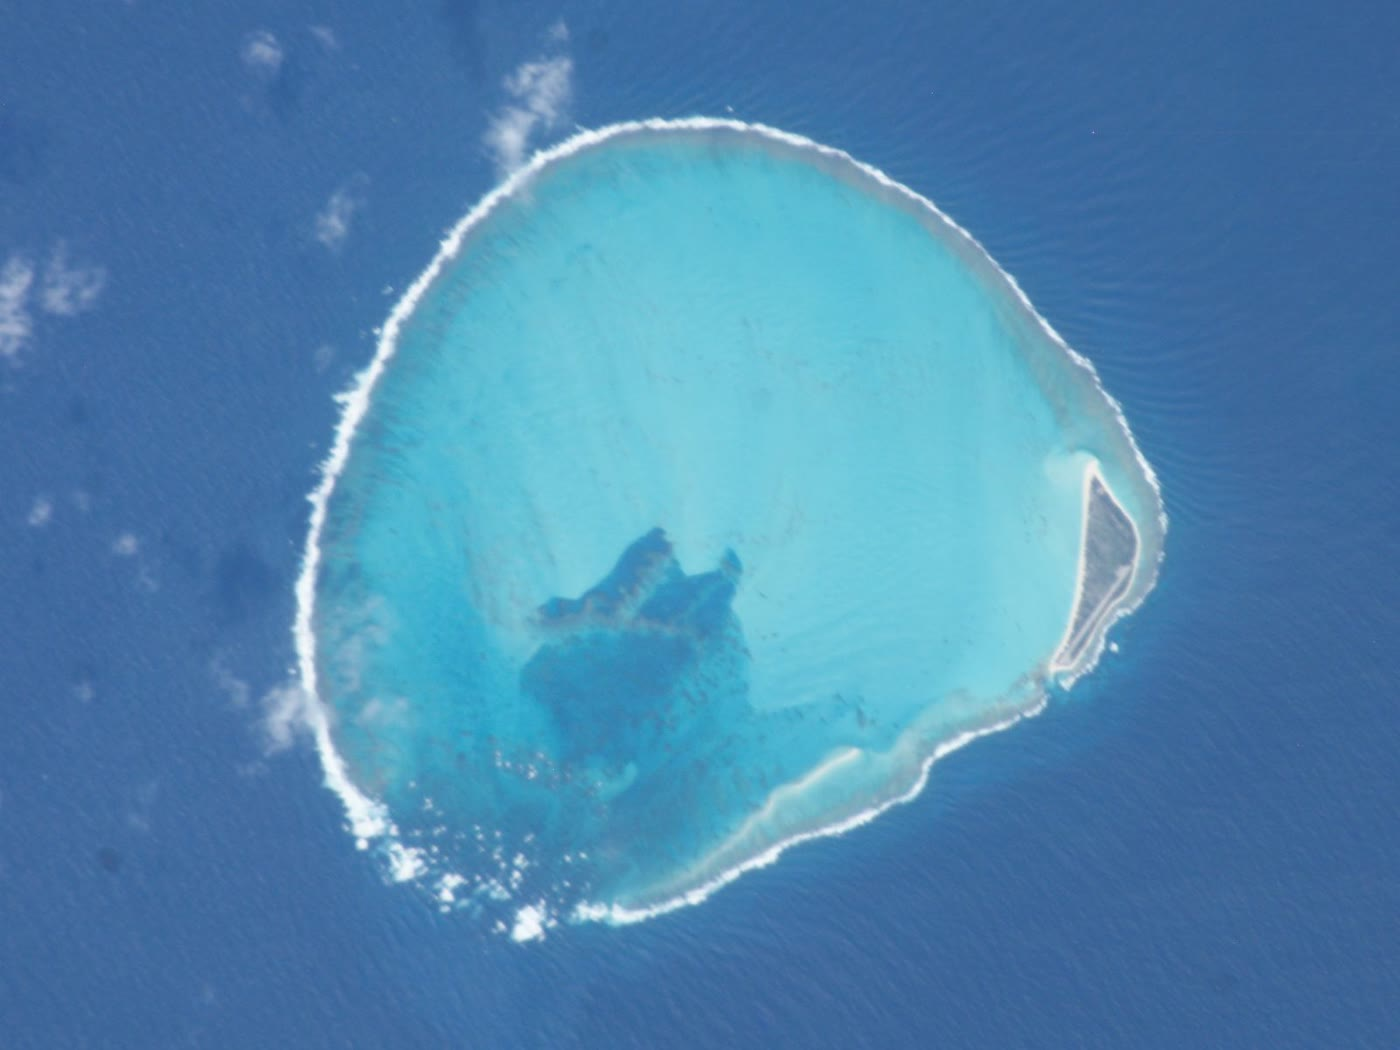
\includegraphics[width=0.52\linewidth]{images/book4/b2-17-kure-atoll.jpg}
\par\smallskip{\small El \omterm{def:b2:oceanic-islands:reefs}{atolón} Kure, el \omterm{def:b2:oceanic-islands:reefs}{atolón} de coral más septentrional, fotografiado por un astronauta desde
la Estación Espacial Internacional el 22 de febrero de 2004. El anillo de arrecife, de unos diez kilómetros de diámetro
como mucho, encierra una laguna; la única isla permanente, Green Island, está en el borde (a la derecha). NASA,
dominio público, a través de Wikimedia Commons.}
\end{omfigure}
% ledger: pmnm:kure (6 miles = 9.7 km)

\section{Erosión, nivel del mar y fin de una isla}\label{sec:b2:oceanic-islands:erosion}

Mientras se hunde, una isla también se desgasta. Una isla alta intercepta los alisios: en las
laderas de barlovento de los volcanes hawaianos caen en algunos lugares más de \qty{9}{m} de lluvia al año.
Los ríos excavan cañones profundos en menos de un millón de años, como en el Kohala, en la isla de Hawái.
Algunos grandes acantilados que se tuvieron por obra exclusiva de la erosión, como los acantilados marinos del norte de
Molokai, se interpretan hoy como las cabeceras de deslizamientos gigantes, retrocedidas desde entonces. El oleaje ataca la costa y
talla a su alrededor una plataforma de abrasión al nivel del mar. Erosión y hundimiento juntos eliminan todo rastro
de roca volcánica sobre el mar en unos \qty{15}{Myr}. Gardner Pinnacles, de aproximadamente esa edad, es
la isla más antigua de la cadena en la que todavía asoma roca volcánica sobre el agua. Más allá, hacia el
noroeste, solo hay islas de arena, atolones y volcanes ahogados.
% ledger: cs14:erosion, cs14:erase

El nivel del mar no permanece quieto mientras tanto. Durante el último máximo glacial estaba unos
\qty{120}{m} más bajo que hoy. La costa de una isla estaba entonces más abajo en sus flancos, y los arrecifes
que hoy la orlan eran tierra firme. Cuando se fundió el hielo, el mar subió una media de \qty{12}{m}
cada mil años durante la deglaciación principal, de 16.5 a \qty{8.2}{ka}. Durante el pulso de agua de deshielo
1A subió al menos \qty{40}{mm} al año. Un arrecife sobre un volcán que se hunde debe seguir ambas
subidas. Frente a la costa noroeste de la isla de Hawái, al menos seis arrecifes ahogados forman una
escalera en el flanco, el más antiguo el más profundo. Cada uno creció en la orilla, se quedó atrás durante una subida
del mar y fue arrastrado hacia abajo por la carga de la isla joven. Una vez que un volcán se ha hundido más
de unos \qty{125}{m}, la amplitud del nivel del mar glacial, ya no volverá a subir hasta el oleaje.
% ledger: usgs:lgm (Book 1), lambeck14:lgm (Book 2), cs14:erase, cs14:subsidence

El arco puede actuar en sentido contrario. Oahu se asienta sobre el abombamiento levantado por la carga de las islas más jóvenes,
y se ha elevado un poco: arrecifes del último interglacial, de 133 a \qty{115}{ka}, afloran alrededor de toda
la isla, y un arrecife de unos \qty{334}{ka} se encuentra hoy \qty{21}{m} sobre el nivel del mar. El
fin de una \omterm{def:b2:oceanic-islands:stages}{isla oceánica} queda así escrito en sus rocas y sus arrecifes. La lava la construye, los deslizamientos y
la lluvia la desmantelan, el oleaje la arrasa, la placa la hunde, y un arrecife mantiene su lugar en la
superficie hasta que el agua fría y un mar que sube lo ahogan también.
% ledger: cs14:arch

\section*{Ejercicios}\label{sec:b2:oceanic-islands:exercises}

Datos para los ejercicios, salvo indicación contraria: ley profundidad--edad $d = \qty{2500}{m} + C\sqrt t$ con
$C = \qty{350}{m.Myr^{-1/2}}$ para $0 \le t \le \qty{70}{Myr}$, y $d = \qty{6400}{m} -
\qty{3200}{m}\,e^{-t/62.8}$ más allá de \qty{20}{Myr}; $1~\text{pie} = \qty{0.3048}{m}$, $1~\text{braza}
= \qty{1.8288}{m}$, $1~\text{milla} = \qty{1.609}{km}$; crecimiento arrecifal de hasta \qty{4.2}{mm.yr^{-1}}.

\begin{exercise}[$\star$]\label{exo:b2:oceanic-islands:1}
Nómbrese la etapa de cada volcán: (a) un \omterm{def:b2:oceanic-islands:seamount}{monte submarino} cuya cima está a \qty{975}{m} bajo el mar y que emite
lava alcalina; (b) un volcán sobre el punto caliente que emite lava toleítica a un ritmo alto; (c) un
volcán extinto cuyas últimas coladas, más alcalinas que el grueso de la isla, recubren el escudo; (d) una
isla en la que, tras un silencio de \qty{2}{Myr}, se abren unas pocas bocas alcalinas pequeñas; (e) un anillo de arrecife
alrededor de una laguna sin roca volcánica a la vista.
\end{exercise}

\begin{exercise}[$\star$]\label{exo:b2:oceanic-islands:2}
Un volcán se construye sobre una placa de \qty{9}{Myr}. (a) ¿A qué profundidad está el fondo marino a su alrededor? (b) ¿Cuánto
se habrá hundido cuando la placa tenga \qty{25}{Myr}? (c) ¿A qué velocidad se hunde entonces?
\end{exercise}

\begin{exercise}[$\star$]\label{exo:b2:oceanic-islands:3}
Diecisiete grandes deslizamientos se formaron en los últimos \qty{5}{Myr} alrededor de las islas Hawái principales, y
setenta a lo largo de la cordillera de Hawái en \qty{30}{Myr}. (a) Hállese el intervalo medio entre dos deslizamientos en
cada caso. (b) ¿Por qué ambos son solo cotas superiores del intervalo verdadero?
\end{exercise}

\begin{exercise}[$\star$]\label{exo:b2:oceanic-islands:4}
En Enewetak se encontró basalto a 4158 pies en un sondeo y basamento duro a 4610 pies en el
otro; los corales de arrecife de la base de la caliza no viven a más de 150 pies de profundidad. (a) Conviértanse
las tres profundidades a metros. (b) ¿Cuánto se ha hundido como mínimo la cima del volcán bajo la isla Parry
desde que creció en ella el primer arrecife? (c) La base de la caliza es eocena, así que tiene al menos
\qty{33.9}{Myr}. ¿Cuál es la mayor velocidad media de hundimiento posible?
\end{exercise}

\begin{exercise}[$\star\star$]\label{exo:b2:oceanic-islands:5}
(a) Hállese la velocidad de hundimiento térmico, en \unit{m} por \unit{Myr} y en \unit{mm.yr^{-1}}, de
islas sobre placas de 4, 25 y \qty{49}{Myr}. (b) ¿Cuántas veces más deprisa que la más rápida de ellas
puede crecer un arrecife productivo? (c) ¿Y cuántas veces más rápida es la fase de carga frente a la isla de
Hawái, \qty{2.6}{m} por cada mil años?
\end{exercise}

\begin{exercise}[$\star\star$]\label{exo:b2:oceanic-islands:6}
(a) Con la ley exponencial, hállese la velocidad de hundimiento sobre una placa de \qty{100}{Myr}, en \unit{m}
por cada mil años, y compárese con los \qty{0.01}{m} por cada mil años medidos a lo largo de la
cordillera de Hawái. (b) ¿Para qué edad de la placa la velocidad es exactamente \qty{10}{m.Myr^{-1}}? (c) Compruébese que las
dos leyes dan casi la misma profundidad para una placa de \qty{25}{Myr}.
\end{exercise}

\begin{exercise}[$\star\star$]\label{exo:b2:oceanic-islands:7}
Los arrecifes hawaianos se ahogan unos \qty{33}{Myr} después del nacimiento de su volcán, y el volcanismo avanza
a lo largo de la cadena a \qty{8.6}{cm.yr^{-1}}. (a) ¿A qué distancia del punto caliente está una isla cuando su
arrecife se ahoga? (b) Midway es un \omterm{def:b2:oceanic-islands:reefs}{atolón} de \qty{27.7}{Myr}: ¿es coherente que todavía tenga un
arrecife vivo? (c) Kure está 55 millas más allá de Midway. Estímese su edad y dígase si está cerca
del \omterm{def:b2:oceanic-islands:darwin-point}{punto de Darwin}.
\end{exercise}

\begin{exercise}[$\star\star$]\label{exo:b2:oceanic-islands:8}
En la \omterm{def:b2:oceanic-islands:collapse}{avalancha de derrubios} de Nuuanu, el \omterm{def:b2:oceanic-islands:seamount}{monte submarino} Tuscaloosa es un bloque de unos \qty{30}{km} de largo,
\qty{17}{km} de ancho y al menos \qty{2}{km} de alto. (a) ¿Qué volumen tendría una caja de esas dimensiones?
¿Y una pirámide de la misma base y la misma altura? (b) Compárese con el volumen del
Kilauea, \qty{10000}{km^3}. (c) La avalancha cubre \qty{23000}{km^2}. Si tuviera un espesor medio de
\qty{100}{m} (una hipótesis: su espesor lejos de Oahu se conoce mal), ¿cuál sería su
volumen?
\end{exercise}

\begin{exercise}[$\star\star$]\label{exo:b2:oceanic-islands:9}
Frente a la isla de Hawái el flanco se hunde \qty{2.6}{m} por cada mil años bajo la carga del
volcán. (a) ¿Cuánto se tarda en ahogar una línea de costa \qty{1}{km}? (b) Un arrecife que crece a
\qty{4.2}{mm.yr^{-1}} está sobre este flanco. ¿Sigue el ritmo con el nivel del mar estable? (c) Durante la
deglaciación principal, de 16.5 a \qty{8.2}{ka}, el mar subió \qty{12}{mm.yr^{-1}} de media. ¿A qué
profundidad queda el techo del arrecife al final, si empezó en la superficie? (d) Lo mismo para un arrecife sobre
un volcán antiguo que ya no se hunde.
\end{exercise}

\begin{exercise}[$\star\star\star$]\label{exo:b2:oceanic-islands:10}
(a) Demuéstrese que, en un intervalo fijo $\Delta$, la ley de la raíz hace que una isla se hunda menos cuanto más vieja es su
placa. (b) Calcúlese el hundimiento en \qty{20}{Myr} para una isla nacida en la dorsal y para otra nacida
sobre una placa de \qty{50}{Myr}. (c) La placa bajo una dorsal está muy caliente, y la ley de la raíz da una
velocidad infinita en $t = 0$. ¿Es un problema para el hundimiento en un intervalo finito? Explíquese.
\end{exercise}

\begin{exercise}[$\star\star\star$]\label{exo:b2:oceanic-islands:11}
Un \omterm{def:b2:oceanic-islands:reefs}{atolón} se hunde a \qty{30}{m.Myr^{-1}}, y el nivel del mar oscila unos \qty{120}{m} con las
glaciaciones, en ciclos de unos \qty{100}{kyr}. (a) ¿Cuánto se hunde el \omterm{def:b2:oceanic-islands:reefs}{atolón} durante un ciclo? (b) En un
nivel bajo glacial, ¿a qué altura sobre el mar queda el techo del \omterm{def:b2:oceanic-islands:reefs}{atolón}? ¿Qué le ocurre entonces a la
roca arrecifal? (c) ¿Cuántos ciclos hacen falta para que el \omterm{def:b2:oceanic-islands:reefs}{atolón} se hunda los \qty{120}{m} completos?
(d) Explíquense las zonas lixiviadas halladas en los sondeos de Enewetak, y por qué la
\cref{prop:b2:oceanic-islands:cap} sigue dando el espesor del casquete a largo plazo.
\end{exercise}

\begin{exercise}[$\star\star\star$]\label{exo:b2:oceanic-islands:12}
Un \omterm{def:b2:oceanic-islands:reefs}{atolón} se ahoga cuando su placa tiene \qty{50}{Myr}: su arrecife se queda atrás y su techo acaba en el
límite de crecimiento de las algas coralinas más profundas, \qty{150}{m} bajo el mar. (a) Con la ley
exponencial, ¿cuánto más se hunde antes de que la placa tenga \qty{120}{Myr}? (b) ¿A qué profundidad está entonces
la cima del \omterm{def:b2:oceanic-islands:seamount}{guyot}? (c) Un \omterm{def:b2:oceanic-islands:seamount}{guyot} junto a Enewetak tiene su cima a 700 brazas. Conviértase y compárese.
(d) Nómbrense dos razones por las que un \omterm{def:b2:oceanic-islands:seamount}{guyot} real podría ser más profundo o más somero que esta estimación.
\end{exercise}

\begin{problem}[{Problema de fin de semana --- Del volcán al atolón}]\label{pb:b2:oceanic-islands:1}
La isla inventada de Petrel nace sobre un punto caliente en una placa de \qty{10}{Myr}. Su volcán es
un cono de \qty{50}{km} de radio basal. Cuando termina su crecimiento, su cima está \qty{1000}{m} sobre el
nivel del mar. Su última roca volcánica desaparece bajo el nivel del mar \qty{12}{Myr} después. Un arrecife
mantiene entonces su techo al nivel del mar hasta que la placa tiene \qty{70}{Myr}, cuando el \omterm{def:b2:oceanic-islands:reefs}{atolón} cruza el
\omterm{def:b2:oceanic-islands:darwin-point}{punto de Darwin}. Úsense la ley profundidad--edad de los ejercicios (la ley de la raíz hasta \qty{70}{Myr}, la
ley exponencial a partir de ahí), un crecimiento arrecifal de \qty{4.2}{mm.yr^{-1}} y los datos del capítulo.
El nivel del mar se toma constante, salvo en las preguntas 8 a 10. Las profundidades se redondean al metro.

\noindent\textbf{Parte I --- Crecimiento.}
\begin{enumerate}
  \item ¿A qué profundidad está el fondo marino donde nace Petrel?
  \item ¿Qué altura tiene el volcán sobre ese fondo cuando termina su crecimiento, despreciando el
        hundimiento del fondo bajo la carga?
  \item Hállese el volumen del cono.
  \item Si el \qty{85}{\percent} se emitió durante una \omterm{def:b2:oceanic-islands:stages}{etapa de escudo} de \qty{1}{Myr}, ¿cuál fue el
        ritmo medio de erupción? Compárese con el aporte actual del Kilauea, unos
        \qty{0.1}{km^3} al año.
  \item ¿Cuántos Petrel harían falta para un Mauna Loa, de \qty{95600}{km^3}?
  \item ¿Qué lavas, toleíticas o alcalinas, forman la mayor parte del cono? ¿Cuáles lo recubren?
\end{enumerate}

\noindent\textbf{Parte II --- Carga y arrecifes ahogados.}
\begin{enumerate}[resume]
  \item Durante su crecimiento, la carga hunde la isla joven \qty{1}{km} en \qty{1}{Myr}. ¿Cuál es
        la velocidad media, y cómo se compara con los \qty{2.6}{m} por cada mil años medidos
        frente a la isla de Hawái?
  \item Un arrecife crece en la orilla durante esta fase, con el nivel del mar estable. ¿Sigue el ritmo, y
        con qué margen?
  \item El nivel del mar sube entonces \qty{12}{mm.yr^{-1}}. ¿Cuánto se queda atrás el arrecife cada
        año?
  \item ¿Cuánto tarda su techo en llegar a \qty{150}{m}, el límite de crecimiento más profundo? ¿Qué
        deja eso en el flanco de la isla?
\end{enumerate}

\noindent\textbf{Parte III --- Hundimiento y erosión.}
\begin{enumerate}[resume]
  \item ¿Cuánto se ha hundido Petrel cuando desaparece su última roca volcánica, si la placa tiene
        entonces \qty{22}{Myr}?
  \item ¿Qué parte de los \qty{1000}{m} de la cima eliminó la erosión, y a qué velocidad media?
  \item ¿A qué velocidad se hunde Petrel cuando termina su crecimiento, y cuando desaparece su cima?
  \item ¿A qué profundidad está entonces el fondo marino a su alrededor?
  \item Compárense los \qty{12}{Myr} que tardó con los \qty{15}{Myr} de las islas Hawái. Dese una
        razón por la que una isla hawaiana alta dura más.
  \item Nómbrense dos procesos, además de la lluvia y los ríos, que eliminan la isla por encima del nivel del mar.
  \item ¿Qué forma de arrecife rodea Petrel poco antes de que desaparezca su cima?
\end{enumerate}

\noindent\textbf{Parte IV --- Atolón y guyot.}
\begin{enumerate}[resume]
  \item ¿Qué espesor tiene el casquete arrecifal cuando la placa tiene \qty{70}{Myr}?
  \item ¿Qué velocidad media de crecimiento arrecifal hizo falta? ¿Cuántas veces menor es que el crecimiento
        que podría alcanzar el arrecife?
  \item Compárese el casquete con la profundidad del basalto bajo Enewetak.
  \item ¿A qué profundidad está el fondo marino alrededor del \omterm{def:b2:oceanic-islands:reefs}{atolón} cuando cruza el \omterm{def:b2:oceanic-islands:darwin-point}{punto de Darwin}?
  \item Con la ley exponencial, ¿cuánto más se hunde el \omterm{def:b2:oceanic-islands:reefs}{atolón} ahogado antes de que la placa tenga
        \qty{120}{Myr}?
  \item Si el techo del arrecife se detuvo a \qty{150}{m} al ahogarse, ¿a qué profundidad está entonces la cima del
        \omterm{def:b2:oceanic-islands:seamount}{guyot}?
  \item En resumen: ¿qué espesor tiene el casquete arrecifal del \omterm{def:b2:oceanic-islands:reefs}{atolón} de Petrel?
\end{enumerate}
\end{problem}
